\chapter[Overview]{Overview of the Project}
\minitoc

\section{Introduction}
In the realm of software development and design, the creation of UML diagrams plays a crucial role in visualizing system structures and workflows. These diagrams facilitate understanding among team members and stakeholders, enabling better communication and efficient project execution. However, traditional methods of creating UML diagrams using graphical interfaces often prove to be time-consuming and cumbersome. The advent of textual tools such as PlantUML, Mermaid, and Graphviz has streamlined the process, allowing developers to generate diagrams through simple code. This project aims to revolutionize the process further by integrating artificial intelligence to create an innovative platform for generating UML diagrams based on textual commands.

\section{Overview of the Host Organization}
% This section is skipped for now.

\section{Presentation of the Project Context}

\subsection{Problem Statement}
Creating UML diagrams using graphical interfaces demands considerable manual effort, often leading to inefficiencies and errors. These platforms require users to place and adjust elements manually, which can be a tedious process, especially for large or complex diagrams. Alternatively, textual tools like PlantUML, Mermaid, and Graphviz have simplified the creation process by enabling diagram generation through code. However, these tools still demand familiarity with specific syntax, limiting their accessibility to non-technical users.

Moreover, these platforms lack intuitive interfaces that bridge the gap between textual commands and visual representations. The absence of AI-powered features to infer user intent from concise descriptions further complicates the diagram creation process. As a result, there is a significant need for a user-friendly, intelligent platform that caters to both technical and non-technical users.

\subsection{Existing Solutions}
Several existing solutions address the need for textual UML diagram generation. Prominent tools in this domain include:

\begin{itemize}
    \item \textbf{PlantUML:} A robust tool that allows users to generate UML diagrams from textual descriptions using a straightforward syntax. It supports a wide variety of diagrams but requires users to learn its syntax.
    \item \textbf{Mermaid:} A modern diagramming tool that integrates seamlessly with markdown. While it provides an accessible syntax, its feature set is more limited compared to PlantUML.
    \item \textbf{Graphviz:} A versatile tool primarily focused on graph visualization. It offers powerful features but lacks the domain-specific focus for UML diagrams.
    \item \textbf{Diagramming AI:} A recent AI-powered tool that interprets natural language inputs to generate diagrams. However, its capabilities are still in development, and customization options remain limited.
    \item \textbf{ChatUML:} An innovative platform leveraging AI to assist users in creating UML diagrams. While promising, it often struggles with complex requirements.
\end{itemize}

\subsection{Proposed Solution}
The proposed platform aims to overcome the limitations of existing solutions by combining the precision of textual tools with the adaptability of artificial intelligence. Users can input concise descriptions or specific requirements, and the platform will generate accurate and ready-to-use UML diagrams. Key features include:

\begin{itemize}
    \item Integration of AI to interpret user intents from natural language descriptions.
    \item A user-friendly interface that dynamically converts textual commands into diagrams.
    \item Support for sharing and collaboration, fostering a community of diagram creators.
\end{itemize}

\subsubsection{Use of PlantUML}
PlantUML was chosen as the core engine for diagram generation due to its:

\begin{itemize}
    \item Extensive support for diverse UML diagrams.
    \item Mature ecosystem and strong community support.
    \item Flexibility and compatibility with various development tools.
\end{itemize}

\begin{table}[h!]
    \centering
    \caption{Comparison of Diagramming Tools}
    \begin{tabular}{|l|l|l|l|}
        \hline
        \textbf{Feature} & \textbf{PlantUML} & \textbf{Mermaid} & \textbf{Graphviz} \\
        \hline
        Diagram Variety & Extensive & Moderate & Limited \\
        Syntax Simplicity & Moderate & High & Low \\
        AI Integration & None (default) & None (default) & None (default) \\
        Community Support & Strong & Growing & Moderate \\
        Integration with Tools & Extensive & Moderate & High \\
        \hline
    \end{tabular}
\end{table}

The choice of PlantUML ensures that our platform is built on a reliable and extensible foundation, while AI integration addresses its limitations in accessibility and usability.




\section{Methodology}
\subsection{Agile Approach}
The development of the platform followed an Agile approach, emphasizing iterative development, collaboration, and adaptability. Agile ensures continuous delivery of functional components, enabling swift feedback incorporation and enhancing the overall quality of the project.

\subsection{Comparison of Agile Methods}
Several Agile methodologies were considered during the project planning phase. Key attributes of these methodologies are outlined in the table below:

\begin{table}[h!]
    \centering
    \caption{Comparison of Agile Methods}
    \begin{tabular}{|l|l|l|l|}
        \hline
        \textbf{Feature} & \textbf{Scrum} & \textbf{Kanban} & \textbf{XP (Extreme Programming)} \\
        \hline
        Iterative Development & Yes & Yes & Yes \\
        Role Definitions & Yes & No & Yes \\
        Visual Workflow Management & Limited & Strong & Limited \\
        Feedback Cycle & Frequent & Continuous & Very Frequent \\
        Suitable for Large Teams & Yes & No & Limited \\
        \hline
    \end{tabular}
\end{table}

Based on this comparison, Scrum was chosen due to its structured framework, adaptability, and emphasis on clear role definitions, making it well-suited for our project's scope and team size.

\subsection{Scrum Framework}
\subsubsection{Key Principles of Scrum}
Scrum operates on principles of transparency, inspection, and adaptation. It ensures that all stakeholders have a clear understanding of the project status and can make informed decisions to address emerging challenges.

\subsubsection{Roles}
Scrum defines distinct roles to streamline responsibilities and collaboration, including the Scrum Master, Product Owner, and Development Team.

\subsubsection{Events}
Scrum incorporates structured events such as Sprint Planning, Daily Standups, Sprint Reviews, and Retrospectives to maintain project momentum and encourage continuous improvement.

\subsubsection{Artifacts}
Key artifacts in Scrum include the Product Backlog, Sprint Backlog, and Increment. These ensure that work remains focused, prioritized, and aligned with project goals.

\section{Modeling Language}
\subsection{Definition}
A modeling language is a standardized system of notations and symbols used to represent the components, relationships, and processes within a system. UML (Unified Modeling Language) stands out as a versatile and widely adopted language for modeling software systems, surpassing other languages like BPMN and ArchiMate in its range of applications.

\subsection{UML Overview}
UML provides a comprehensive suite of diagram types, divided into structural diagrams (e.g., class diagrams, component diagrams) and behavioral diagrams (e.g., activity diagrams, sequence diagrams). These diagrams enable clear communication of system designs and specifications. The following figure illustrates UML's diagram taxonomy:

\begin{figure}[h!]
    \centering
    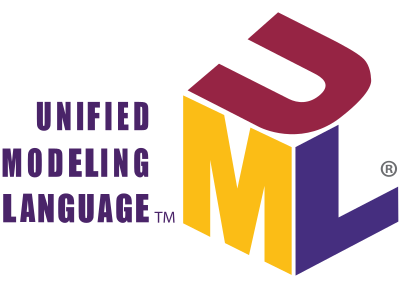
\includegraphics[width=0.8\textwidth]{pictures/web/UML_logo.svg.png}
    \caption{UML 2.5 Diagram Taxonomy}
\end{figure}

\section{Conclusion}
This chapter has provided an overview of the project, highlighting the challenges in current UML diagram generation processes and introducing the proposed solution. The methodology section outlined the Agile approach, emphasizing the reasons for choosing Scrum. Finally, an introduction to UML underscored its significance in system modeling, setting the stage for deeper discussions in subsequent chapters.

